\section{Auswertung}
\label{sec:Auswertung}

\subsection{Horizontalfeldkomponente}

Nachdem der Tisch so ausgerichtet wurde, dass nur die Horizontalkomponente das Magnetfelds\dots 

Somit ergibt sich für das Erdmagnetfeld ein Wert von 
\begin{equation*}
    B_\text{Erdmagnetfeld} = \SI{34.94}{\micro\tesla}.
\end{equation*}
%Formel dafür angeben

\subsection{Landé-Faktoren und Kernspins der Rubidium-Isotope} 

Die gemessenen Werte sind in Tabelle \ref{tab:all}
aufgelistet.
\begin{table}\caption{Die Frequenz ist gegen den Strom der Sweep-Spule und den Strom der Horizontal-Spule für beide Peaks und die resultierenden $B$-Feldstärken aufgetragen.}
    \label{tab:all}
    \centering
    \sisetup{round-mode = places, round-integer-to-decimal=true}
     \begin{tabular}{S[round-precision=1] | S[round-precision=3] S[round-precision=3] S[round-precision=2] | S[round-precision=3] S[round-precision=3] S[round-precision=2]} 
        %\begin{tabular}{c | c c c  | c c c}  
    \toprule
{$f / \si{\kilo\hertz}$} & {$I_\text{sweep,1} / \si{\ampere}$} & {$I_\text{horizontal,1}/ \si{\ampere}$} & {$B_\text{1}/ \si{\micro\tesla}$} & {$I_\text{sweep,2}/ \si{\ampere}$} & {$I_\text{horizontal,2}/ \si{\ampere}$} & {$B_\text{1}/ \si{\micro\tesla}$} \\
\midrule
100     &   0.559   & 0.0       &  33.79 &   0.678 & 0.0         &  40.91  \\
200     &   0.424   & 0.0299    &  51.89 &   0.660 & 0.0299      &  66.13  \\
300     &   0.210   & 0.0599    &  65.29 &   0.567 & 0.0599      &  86.83  \\ 
400     &   0.281   & 0.0749    &  82.73 &   0.754 & 0.0749      &  111.27 \\
500     &   0.267   & 0.0899    &  95.03 &   0.858 & 0.0899      &  130.70 \\
600     &   0.239   & 0.107     &  109.13 &   0.949 & 0.107      &  151.98 \\  
700     &   0.233   & 0.125     &  124.55 &   0.704 & 0.149      &  174.02 \\  
800     &   0.316   & 0.137     &  140.09 &   0.685 & 0.174      &  193.93 \\  
900     &   0.337   & 0.149     &  151.88 &   0.587 & 0.209      &  219.58 \\  
1000    &   0.336   & 0.168     &  167.60 &   0.370 & 0.246      &  238.12 \\    

\bottomrule
\end{tabular}\end{table}

Diese Werte werden mit Formel \eqref{eq:B} in die jeweilige Magnetfeldstärke umgerechnet. %wirklich mit der Formel?
In Abb. \ref{fig:plot} werden die Magnetfeldstärken gegen die Frequenzen aufgetragen und eine Ausgleichsgerade wird durch die Messwerte gelegt. 
\begin{figure}
    \centering
    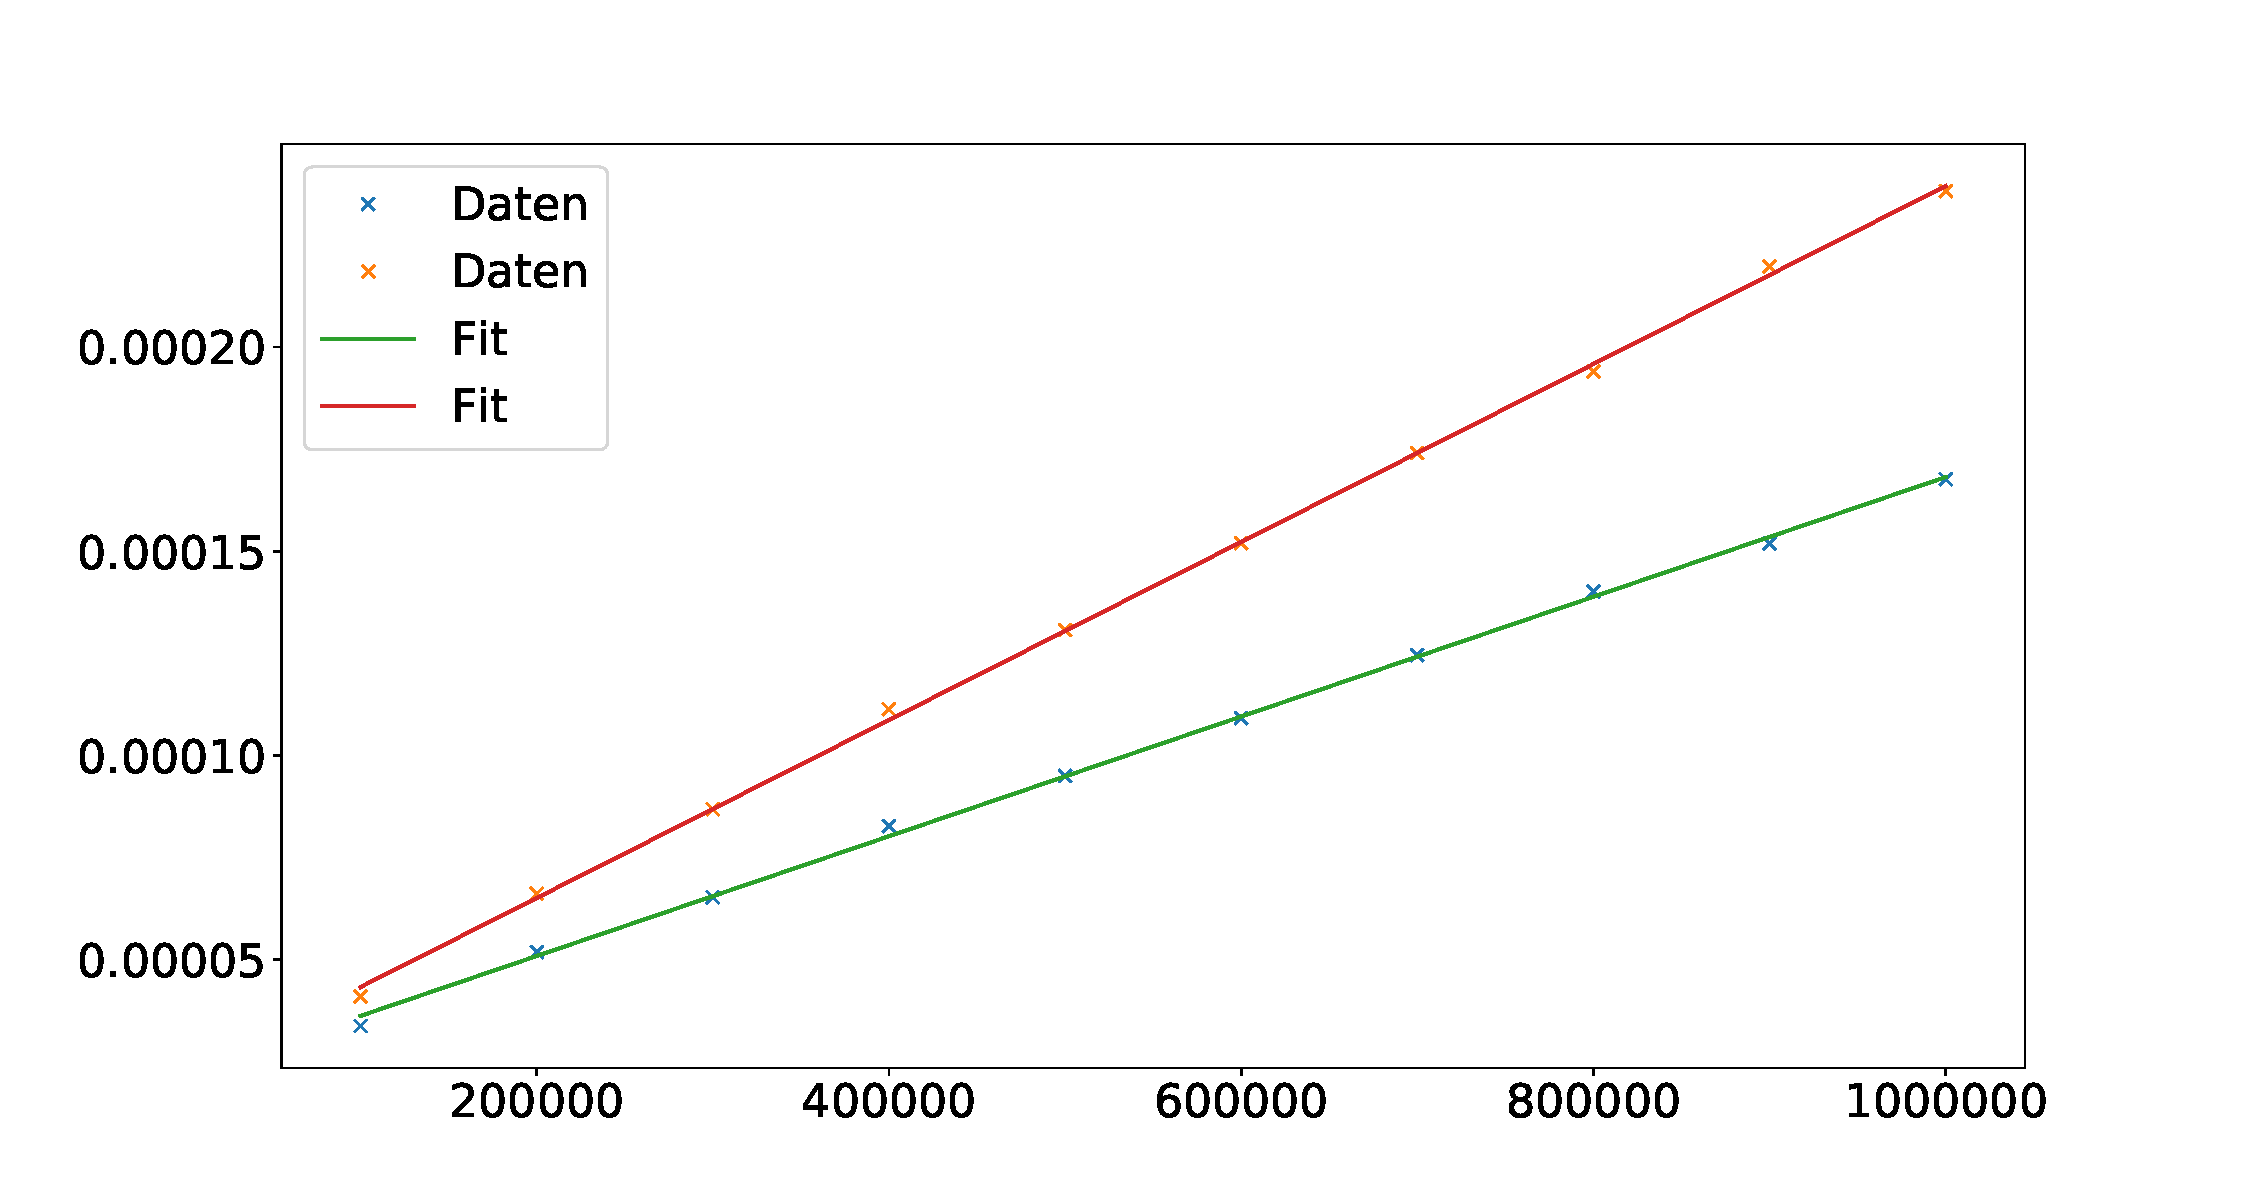
\includegraphics[width=15cm]{plots/fits.pdf}
    \caption{.}
    \label{fig:plot}
\end{figure}

Die Parameter der Ausgleichgeraden haben die folgenden Werte
\begin{align*}
    a_1 &= \SI{1.465e-10}{\tesla\per\hertz} \\ %welche Einheit?
    a_2 &= \SI{2.178e-10}{\tesla\per\hertz} \\
    b_1 &= \SI{2.16e-5}{\tesla} \\
    b_2 &= \SI{2.16e-5}{\tesla}
\end{align*}
Aus der Steigung lässt sich jeweils mit Formel \ref{eq:Zeeman} der Landé-Faktor bestimmen zu
\begin{align*}
    g_{\text{F},1} &= \SI{488 \pm 6}{\meter} \\
    g_{\text{F},2} &= \SI{328 \pm 2.8}{\meter}.
\end{align*}

Aus den Landé-Faktoren lässt sich mit \ref{eq:I} der Kernspin bestimmen zu
\begin{align*}
    I_1 &= \num{1.553} \\
    I_2 &= \num{2.552}.
\end{align*}

Die theoretischen Werte für die Kernspins sind
\begin{align*}
    I_1 &= \frac{3}{2} \\
    I_2 &= \frac{5}{2}.
\end{align*}


\subsection{Isotopenverhältnis}
Aus den beobachteten Amplituden bei $\SI{100}{\kilo\hertz}$, die in Abb. \ref{fig:Aufnahme} zu sehen sind, lässt sich das Isotopenverhältnis ablesen
\begin{equation*}
    \frac{1}{1} = 1. %Werte eintragen
\end{equation*}

In der Natur beträgt das Verhältnis
\begin{equation*}
    \frac{72.168}{27.835} = 2.593.
\end{equation*}

\begin{figure}
    \centering
    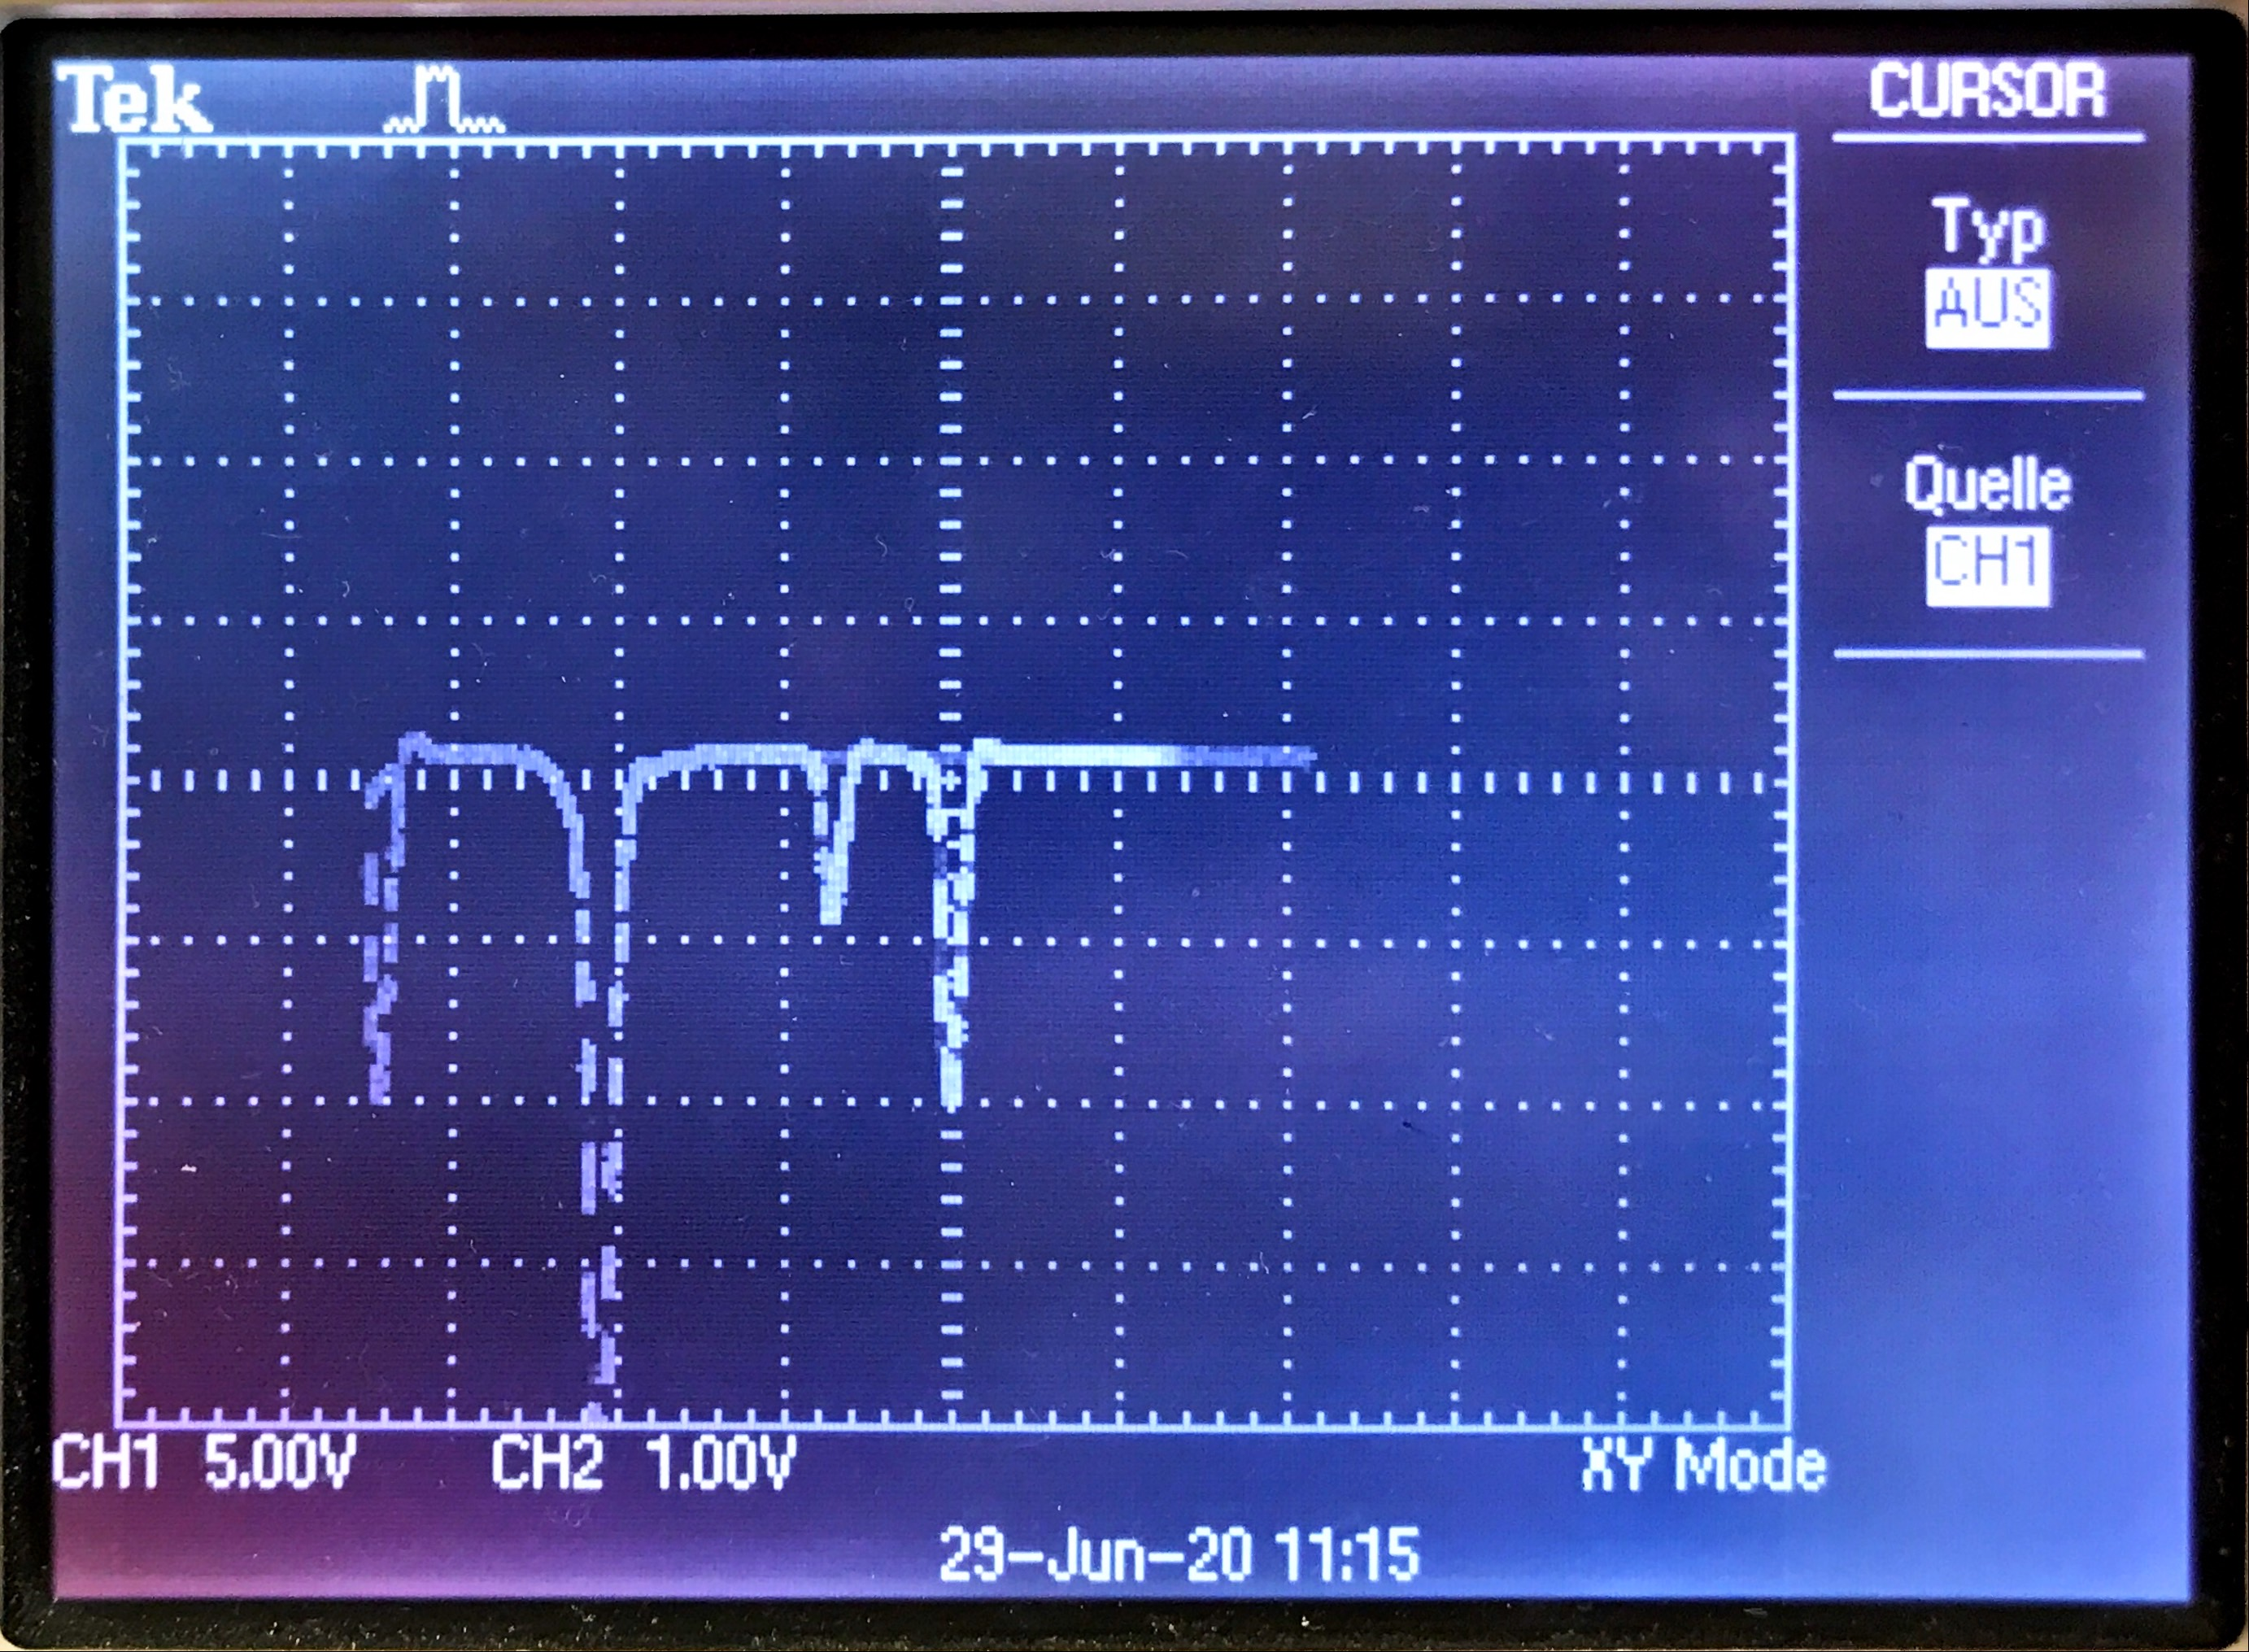
\includegraphics[width=15cm]{fotos/Aufnahme.JPG}
    \caption{Eine typische Aufnahme bei $\SI{100}{\kilo\hertz}$.}
    \label{fig:Aufnahme}
\end{figure}
